\label{4_otimizacao}

Como proposta deste trabalho, pensou-se em como seria possível otimizar um AG de modo a encontrar boas soluções em poucas gerações. Dado o pseudocódigo de um AE, é possível propor uma série de otimizações, desde aquelas voltadas à melhoria de processamento, como o processamento paralelo de indivíduos em uma dada geração, àquelas que otimizam cada uma das quatro operações evolutivas principais (seleção, recombinação, mutação e sobrevivência).

De modo geral, o que traz novas soluções ao problema são as operações de variação (recombinação e mutação), e por conta disso, foram as mais analisadas neste capítulo. Otimizações mais simples discutidas em outros trabalhos, mas que se mostraram eficazes no encontro ou manutenção de boas soluções, também foram discutidas neste capítulo.

A manutenção de boas soluções foi obtida pelo uso de \emph{elitismo}. A otimização nas operações de variação foi obtida pelo uso dos chamados Algoritmos Genéticos Adaptativos (AGA).

\section{Elitismo}

O elitismo é a manutenção do indivíduo mais adaptado de uma geração, deixando-o imune a mutações para que a melhor solução não seja perdida \cite{mitchell1998introduction}. Um indivíduo elitista ainda pode ser considerado para recombinação e geração de filhos, uma vez que as operações de mutação e recombinação são independentes. É possível também criar um grupo elitista, mantendo-se uma certa quantidade ou porcentagem de indivíduos imune a mutações.

Este trabalho utilizou elitismo para o melhor indivíduo em todas as execuções do AG. Tal propriedade pode ser desativada no código.

\section{Algoritmo Genético Adaptativo (AGA)}

A forma mais tradicional de implementação de um AG atribui valores estáticos aos parâmetros de entrada, incluindo os parâmetros de crossover e mutação. No entanto, os indivíduos buscarão soluções de acordo com estes dois parâmetros, e deixá-los estáticos pode limitar o alcance do AG e impedi-lo de encontrar soluções melhores.

Se fosse possível modificar tais parâmetros enquanto o AG é executado, de modo a se adaptar às mudanças de fitness dos próprios indivíduos, teríamos uma solução. Um bom candidato para isso são os chamados Algoritmos Genéticos Adaptivos (AGAs) \cite{srinivas1994adaptive}.

O conceito por trás de um AGA envolve implementar em cima de um AG de modo a modificar os parâmetros de crossover e/ou mutação ao longo do tempo. Não obstante, é possível moldar um AGA de modo a tratar crossover e mutação com probabilidades diferentes para cada indivíduo, de acordo com seus valores de fitness.

Para este trabalho, optou-se por trabalhar com versões adaptadas de outros AGAs \cite{jakobovic1999adaptive, wang2001improved, srinivas1994adaptive} e implementar uma versão própria, explicada a seguir:

\begin{itemize}

	\item Apenas o parâmetro de mutação é modificado ao longo das gerações, uma vez que o crossover seja sempre um valor alto (como 0.9, padronizado neste trabalho);

	\item A adaptação de $p_m$ acontece apenas depois que um ciclo de operações de evolução acontecer;

	\item O que decidirá se $p_m$ mudará será o desvio do melhor valor de fitness $f_{best}$ em comparação com o fitness médio $\bar{f}$, como na equação a seguir:

\begin{equation}
	\left| \frac{f_{best} - \bar{f}}{\bar{f}} \right|
\label{eq:aga}
\end{equation}

	\item Se este desvio for menor que um valor $p{p_m}_0$, isso significa que a mutação está fraca e os indivíduos estão se aproximando de uma mesma solução, que pode não ser necessariamente a melhor. Para contornar isso, $p_m$ irá aumentar;

	\item Caso contrário, as soluções estarão se desviando muito, o que pode ser resultado de uma mutação intensa. Para resolver isso, $p_m$ irá diminuir;

	\item O valor de ${p_m}_0$ é o valor inicial de $p_m$ para o valor inicial de ${p_m}_0$, de modo a servir de termômetro para quão grande deve ser o desvio;

	\item No entanto, $p_m$ não pode ser igual a zero nem maior que 1, dado que representa uma probabilidade. Seguindo a linha de outros trabalhos \cite{matthias2013variable}, $p_m$ será limitado ao intervalo [0.001, 0.5] (se $p_m$ tentar extrapolar estes limites, ele retornará ao valor extremo mais próximo);
	
	\item Mesmo assim, pode acontecer de $p_m$ ficar travado em um dos extremos e o AG não entender o que fazer. Para resolver isto, se $p_m$ ficar travado em um destes limites, ${p_m}_0$ começará a variar na direção oposta. Isto é, se $p_m$ atingir o valor de 0.5, ${p_m}_0$ começará a diminuir em direção ao valor 0.001, e vice-versa.

	\item O incremento/decremento para $p_m$ e ${p_m}_0$ será linear e igual a 0.001;
	
	\item Como há uma divisão por $\bar{f}$, se este valor for zero ou muito próximo de zero para alguma geração, este AGA não será executado.

\end{itemize}

Traduzindo-se a explicação para um algoritmo, chegamos ao código mostrado a seguir. Este trabalho avaliará o desempenho deste AGA comparando a evolução da população com e sem o uso do AGA para um mesmo valor inicial de $p_m$. O intuito não foi o de encontrar um AGA ideal, mas sim o de avaliar se o uso dele ajudaria ou não no encontro de soluções melhores.

\begin{algorithm}[ht]
\Begin{
	${p_m}_0 \gets $ (valor inicial de $p_m$ na inicialização do AG)\;
	$\epsilon \gets 0.0001$\;
	\ForEach{ciclo de operações de evolução} {
		$\bar{f} \gets $ (média dos valores de fitness)\;
		\If{$\bar{f} < \epsilon$} {
			\Return
		}
		$f_{best} \gets $ (melhor valor de fitness na população)\;
		$desvio \gets \left| \frac{f_{best} - \bar{f}}{\bar{f}} \right|$\;
		\If{desvio < ${p_m}_0$} {
			$p_m \gets min(0.5, p_m + 0.001)$\;
			\If{$p_m == 0.5$} {
				${p_m}_0 \gets max(0.001, {p_m}_0 - 0.001)$\;
			}
		}
		\Else{
			$p_m \gets max(0.001, p_m - 0.001)$\;
			\If{$p_m == 0.001$} {
				${p_m}_0 \gets min(0.5, {p_m}_0 + 0.001)$\;
			}
		}
	}
}
\caption{Pseudocódigo do Algoritmo Genético Adaptativo (AGA).}
\label{alg:aga}
\end{algorithm}

A ideia por trás de uma implementação própria foi a de testar a implementação de um AGA a partir de conceitos fáceis de interpretar. Se a ideia de adaptação de um AGA, conforme vista na literatura, for tão simples quanto a base evolutiva do AG, o formato dele também deverá buscar uma implementação simples.

\begin{figure}[ht!]
    \centering 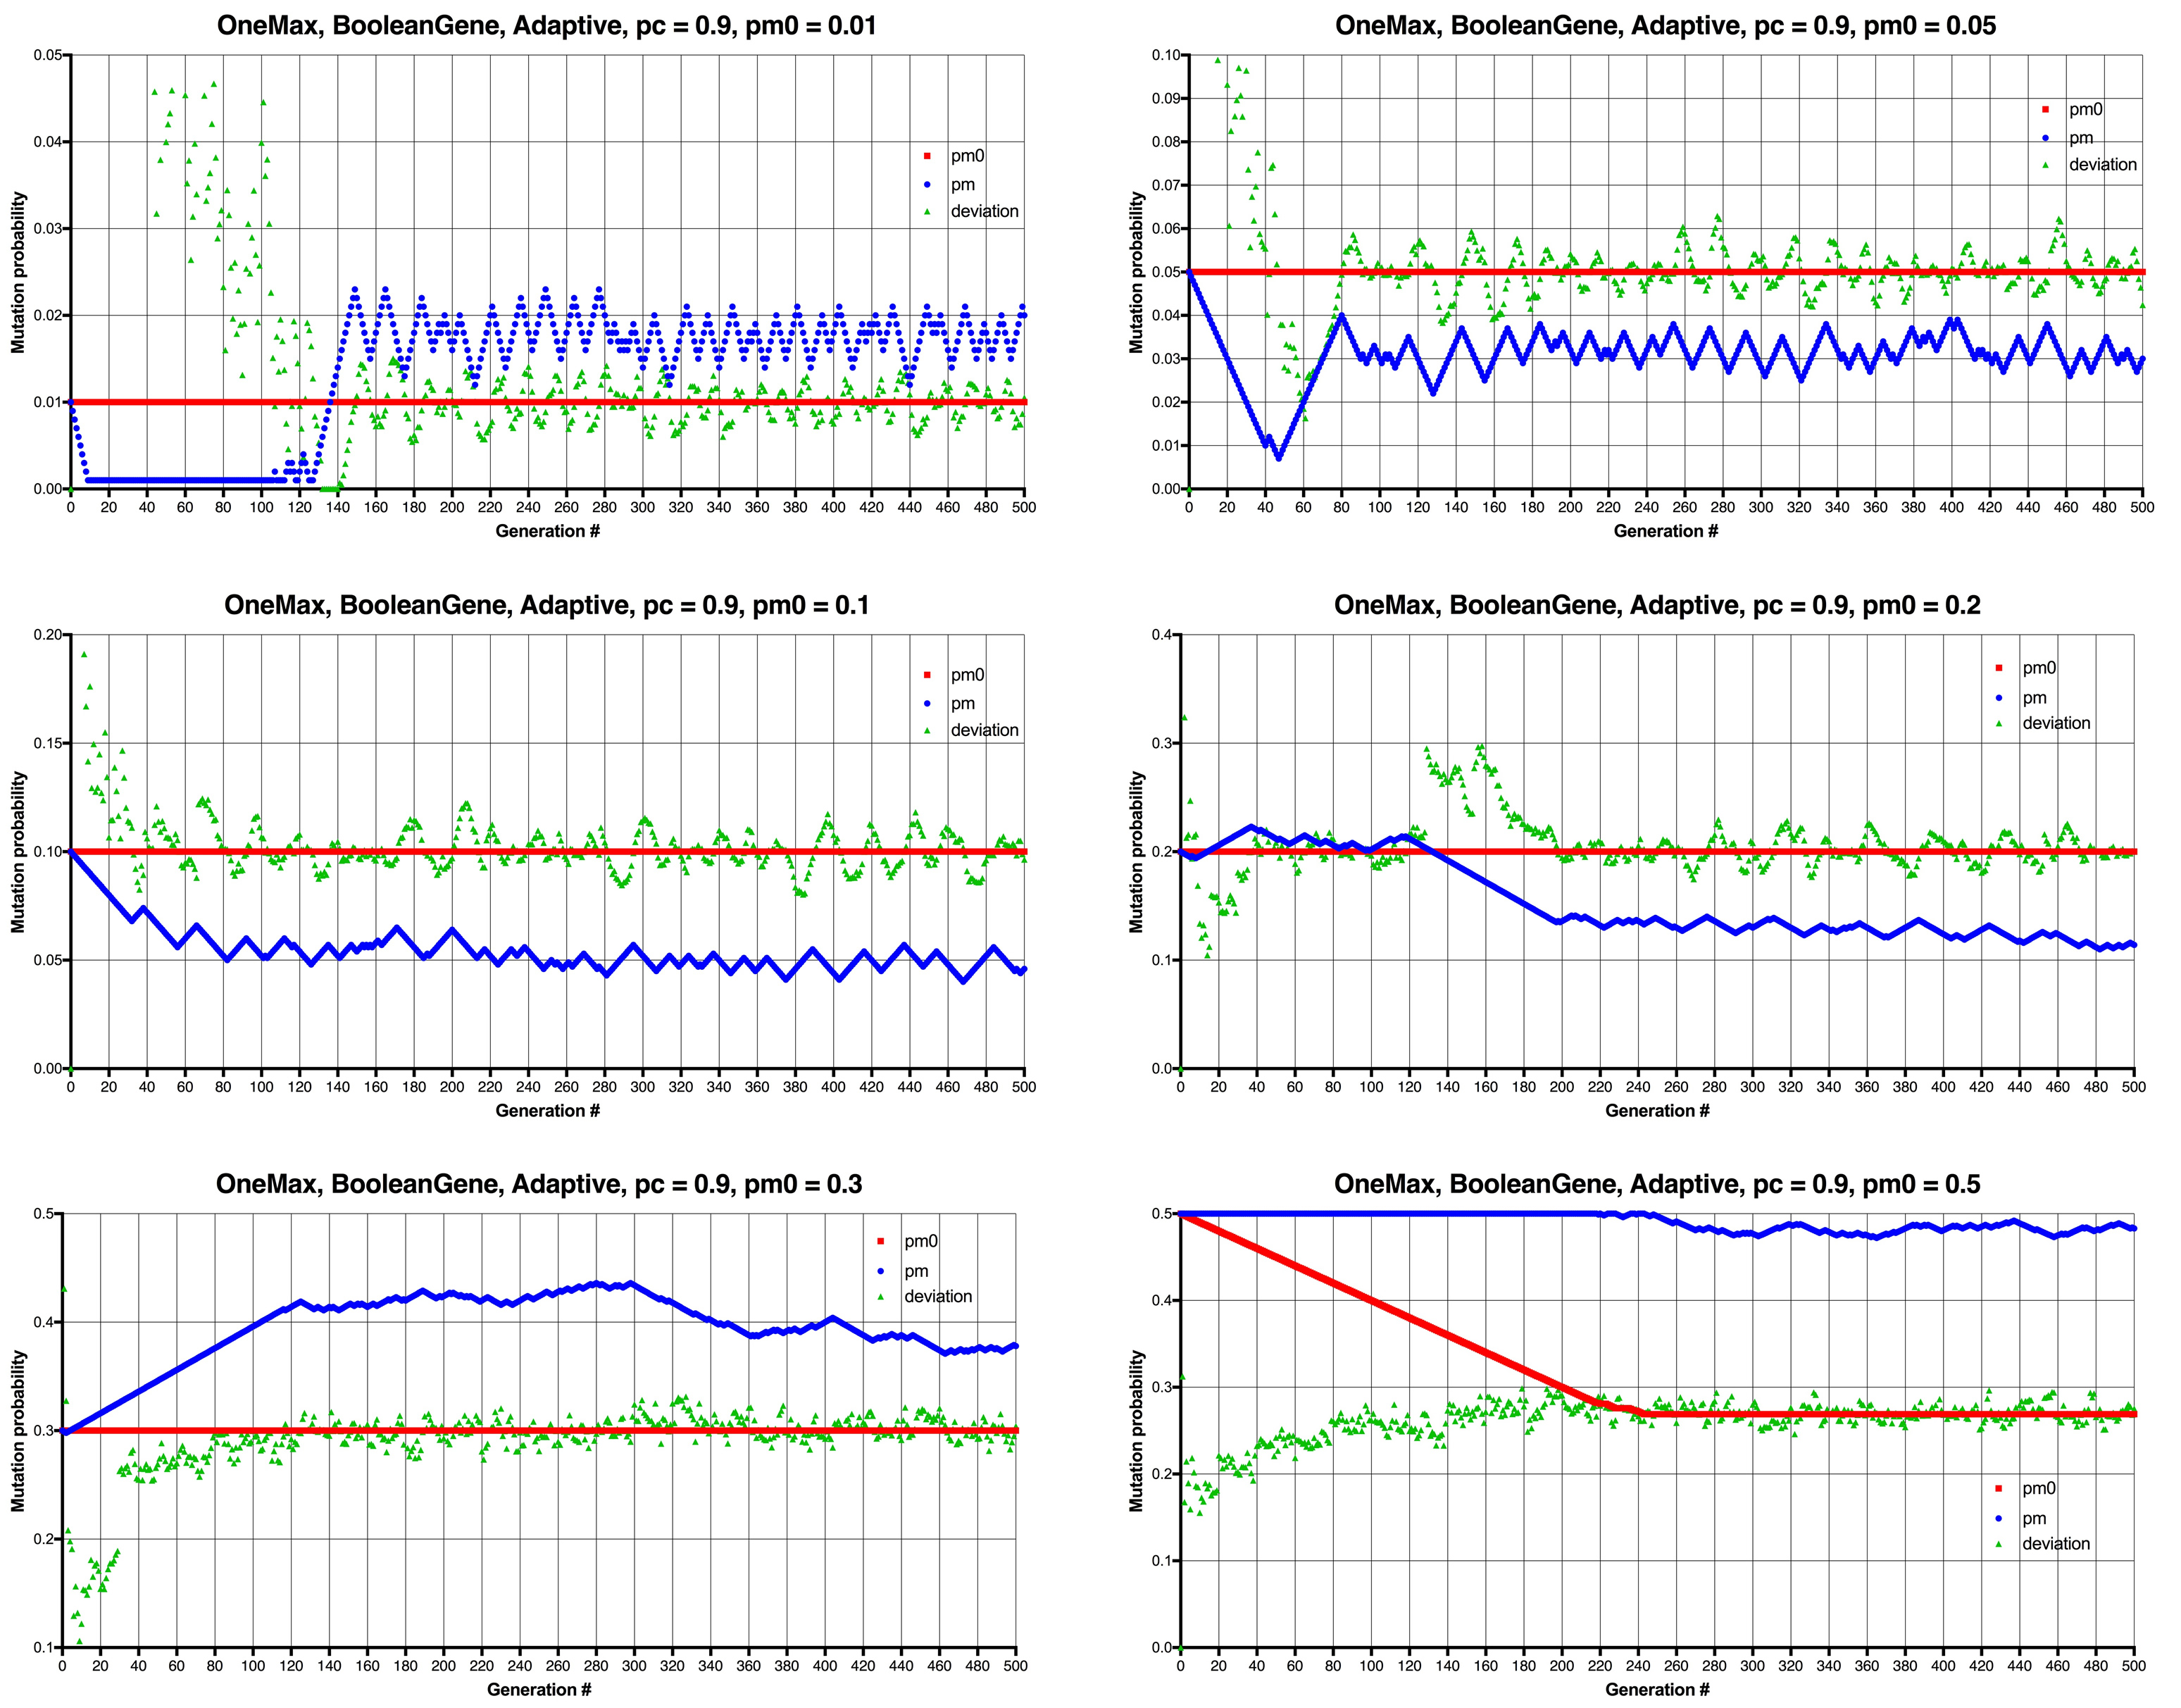
\includegraphics[width=1.0\textwidth]{boolean_onemax_aga.jpg}
    \caption{Evolução dos valores de $p_m$ e ${p_m}_0$ para o problema OneMax para valores diferentes de ${p_m}_0$.}
    \label{fig:aga_test}
\end{figure}
